%!TEX root = ../report.tex
\chapter{Visual Design}\label{ch:visual-design}

To create a visually aesthetic application we have taken into account several preparation steps upfront. In this chapter
we will go into more detail on which steps have been accomplished and how they helped us to implement our frontend parts
later on.

\section{Laws of UX}\label{sec:laws-of-ux}
% TODO @mauritsvanderzee

\section{Styleguide}\label{sec:styleguide}
% TODO @mauritsvanderzee define initial description what styleguides are

\subsection{Grid \& Measurements}\label{subsec:grid-and-measurements}

It started with defining a grid and measurements guide for arranging all application components. For this we created a
grid visualization (Figure~\ref{fig:grid}).

\begin{figure}[!ht]
    \centering
    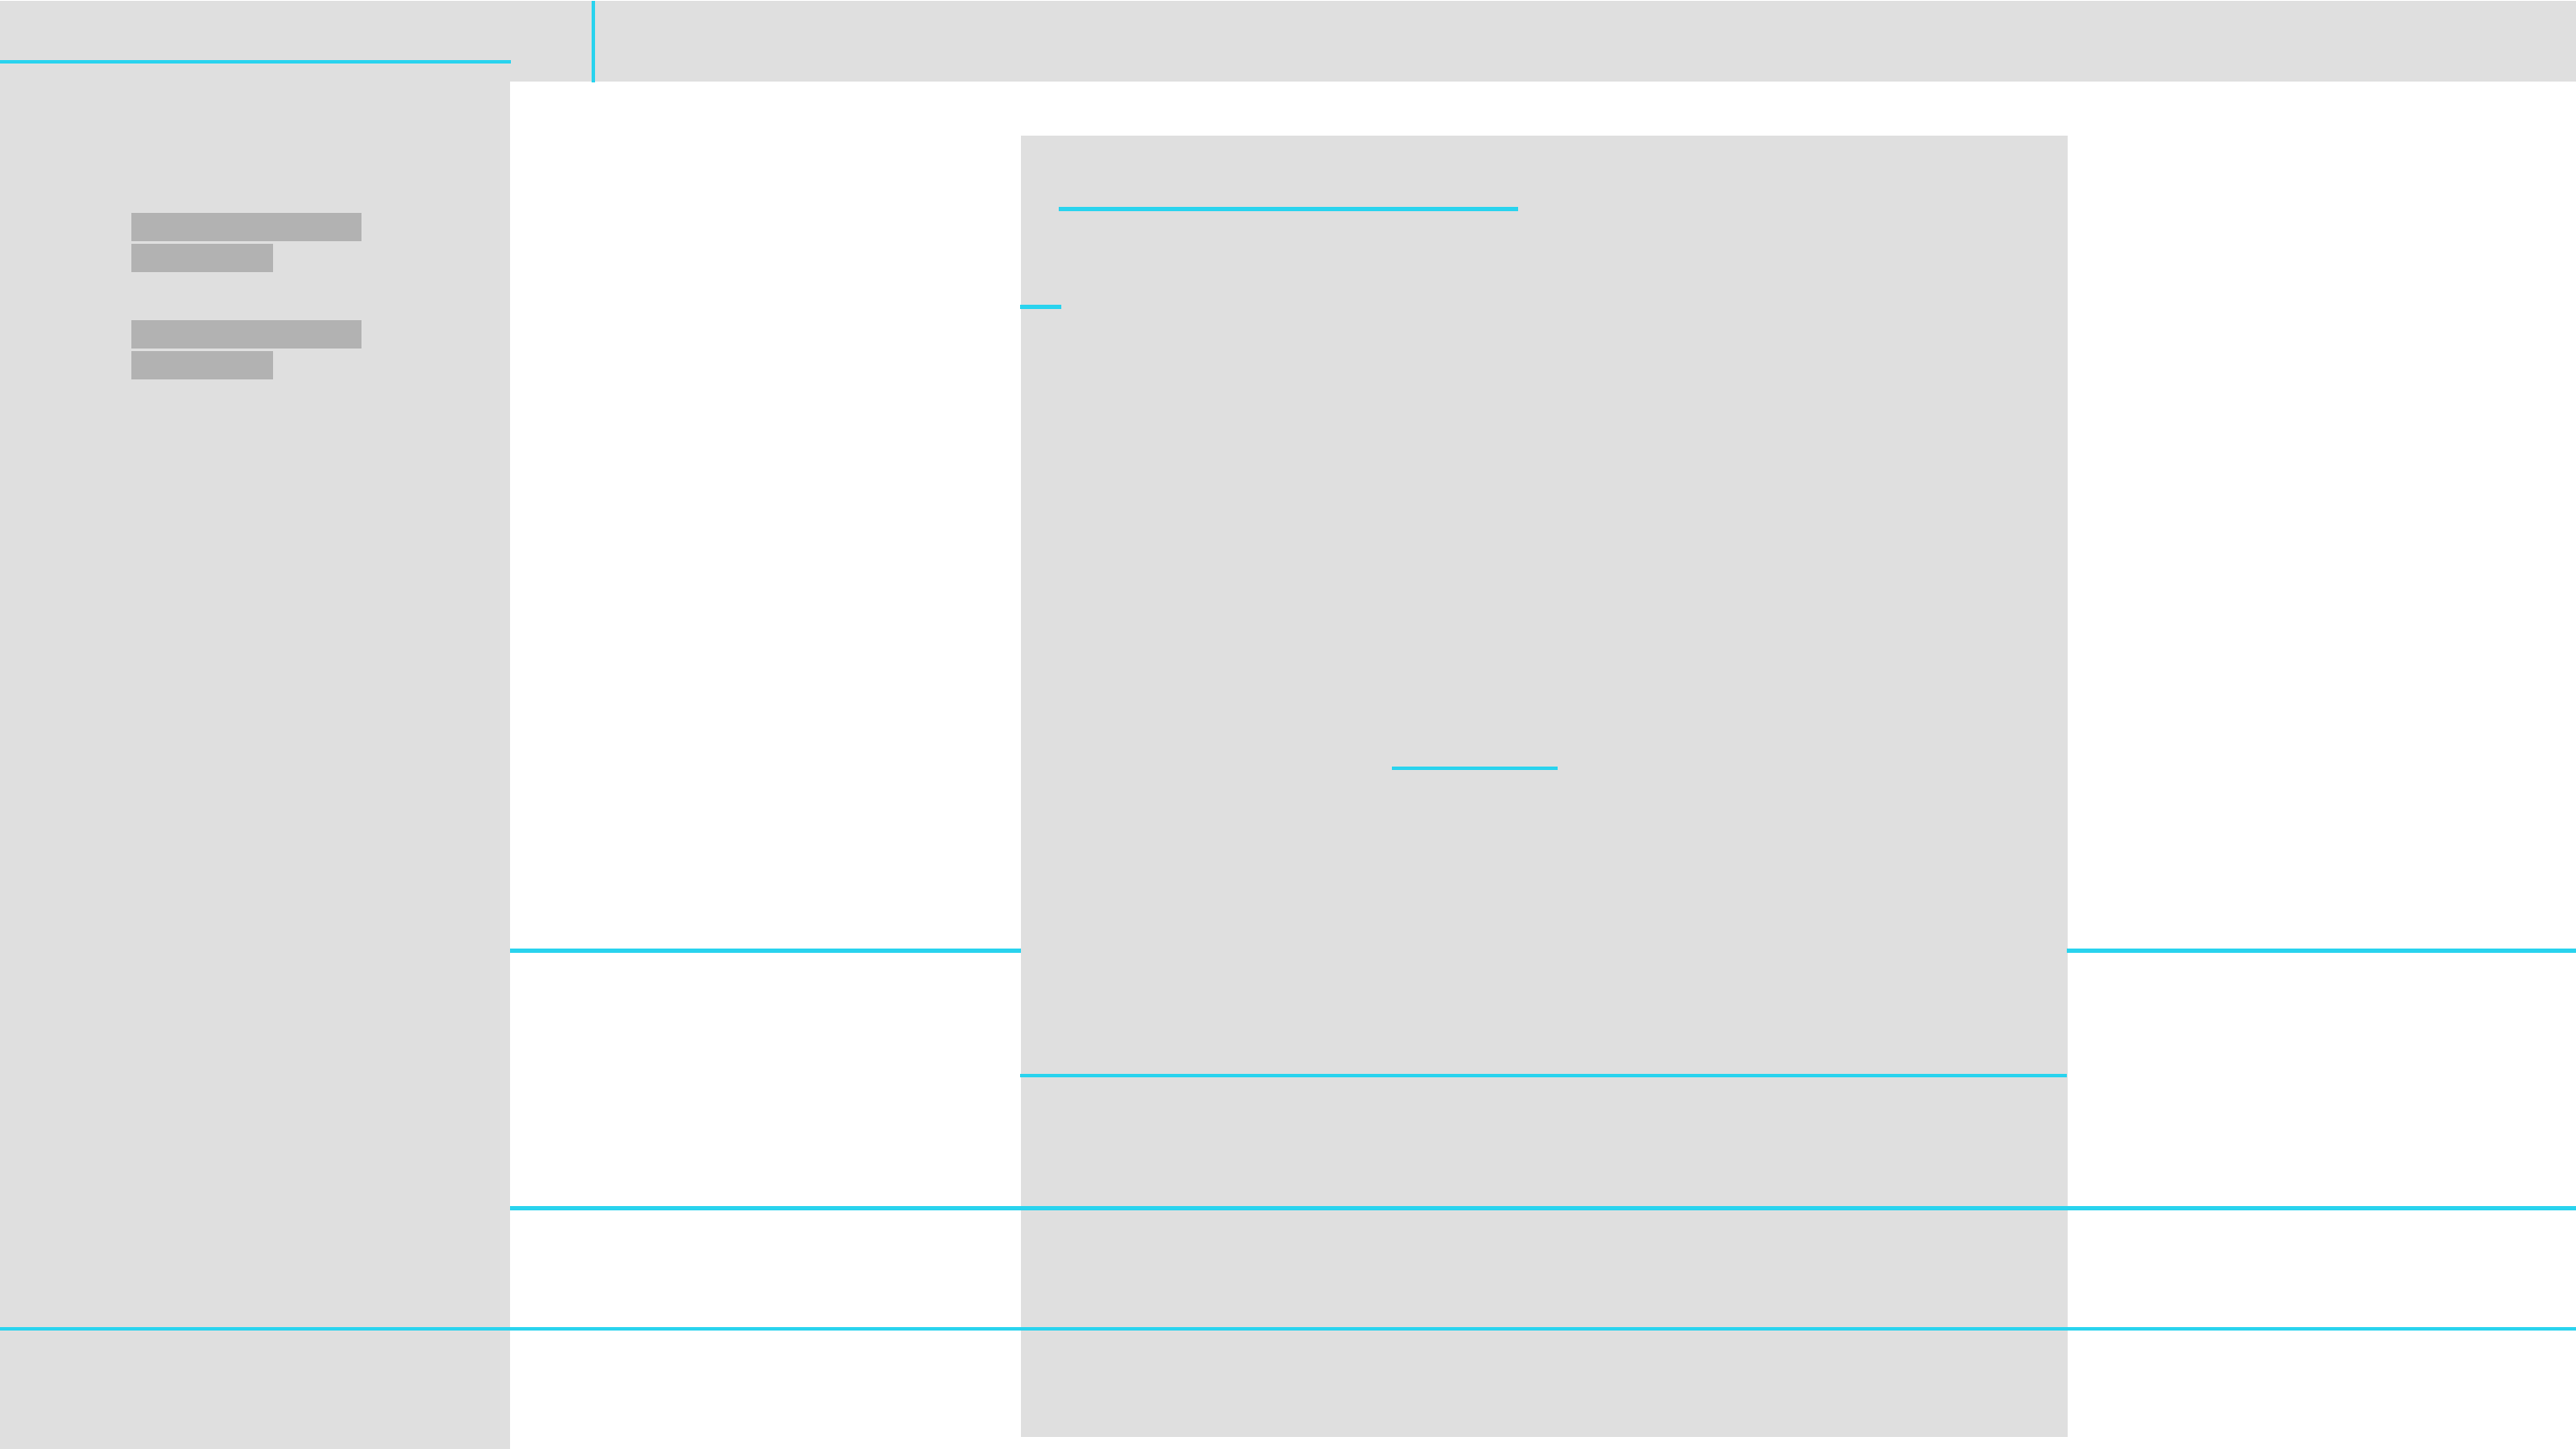
\includegraphics[width=1.0\textwidth]{./images/grid.pdf}
    \caption{Grid and Measurements visualization}
    \label{fig:grid}
\end{figure}

\subsection{Message Styling}\label{subsec:message-styling}

\begin{figure}[ht]
    \caption{Message Styling Design Reference}
    \centering\def\svgwidth{15cm}\input{./graphics/messages.pdf_tex}\label{fig:figure2}
\end{figure}


\subsection{Messages States}\label{subsec:messages-states}
\begin{figure}[ht]
    \caption{Message States Design Reference}
    \centering\def\svgwidth{15cm}\input{./graphics/message-states.pdf_tex}\label{fig:figure3}
\end{figure}

\section{Color Palette}\label{sec:color-palette}

\begin{table}[hb]
    \centering
    \begin{tabular}{|l|l|}
        \hline
        \textbf{Color Name} & \textbf{Hex Code}\\ \hline
        Coral red & \color[HTML]{EE4540}\textbf{\#EE4540} \\ \hline
        French raspberry & \color[HTML]{C72C41}\textbf{\#C72C41} \\ \hline
        Boysenberry & \color[HTML]{801336}\textbf{\#801336} \\ \hline
        Plum violet & \color[HTML]{510A32}\textbf{\#510A32} \\ \hline
        Elderberry & \color[HTML]{21142D}\textbf{\#21142D} \\ \hline
    \end{tabular}
    \caption{List of colors of Trale theme}
    \label{tab:colorTable}
\end{table}

\begin{figure}
    \centering
    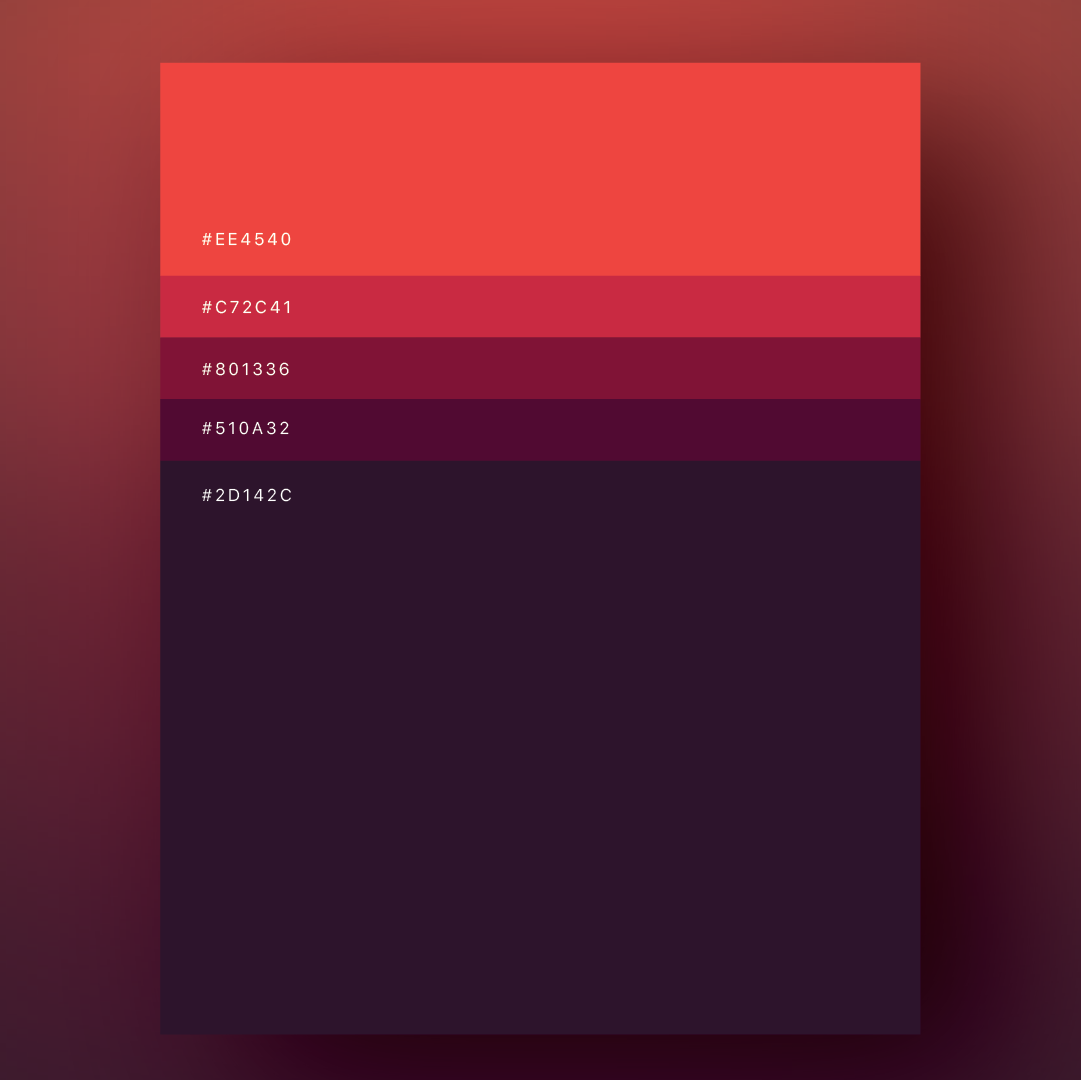
\includegraphics[width=1.0\textwidth]{./images/colorPalette.png}
    \caption{Color Palette of Trale Messenger}
    \label{fig:colorPalette}
\end{figure}

\section{Typography}\label{sec:typography}
% TODO @mauritsvanderzee

\section{Wireframes}\label{sec:wireframes}

Based on our preceding analysis we have created several wireframes which match with our guidelines.
Please refer to our Appendix section for a detailed view of our wireframes. %TODO add link to wireframes appendix
